\chapter{Análise do problema}

Para o elaborar o processo é importante que o problema seja conhecido e consiga ser identificado pelos {\itshape stakeholders} e que a equipe envolvida tenha uma definição comum acerda do problema. A análise do problema é etapa base e fundamental para que os outros processos envolvidos sejam executados, e que o modelo de processo seja condizente com a elaboração do que se refere a soulção.

Foi identificado problemas no processo empíricos envolvidos no controle do estoque e de desperdício, visto que existem situações que não podem ser controladas ou previstas diante de um processo inteiramente humano. Os problemas contidos no processo em questão poderiam ser resolvidos com uma tecnologia apropriada, além de solucionar os defeitos de processos envolvidos, impacta em melhorias gerando menos esforço dos funcionários e mais eficiência no resultado.

\section{Problemas identificados}

Em relação as atividades da empresa identificamos dois principais problemas, através da entrevista e visita ao local, estes são:

\begin{itemize}
	\item Controle de estoque ineficiente;
	\item Falta de controle de desperdício na produção.
\end{itemize}

Para o entendimento dos problemas envolvidos no processo traçamos características relacionadas a estas atividades e assim elaborando um diagrada espinha de peixe ou {\itshape fishbone} para os problemas identificados. O objetivo era traçar o impacto de cada característica das atividades relacionada ao problema e a consequência em que impactava naqquele problema específico.

\subsection{Controle de estoque ineficiente}

\begin{figure}[!htpb]
		\centering
		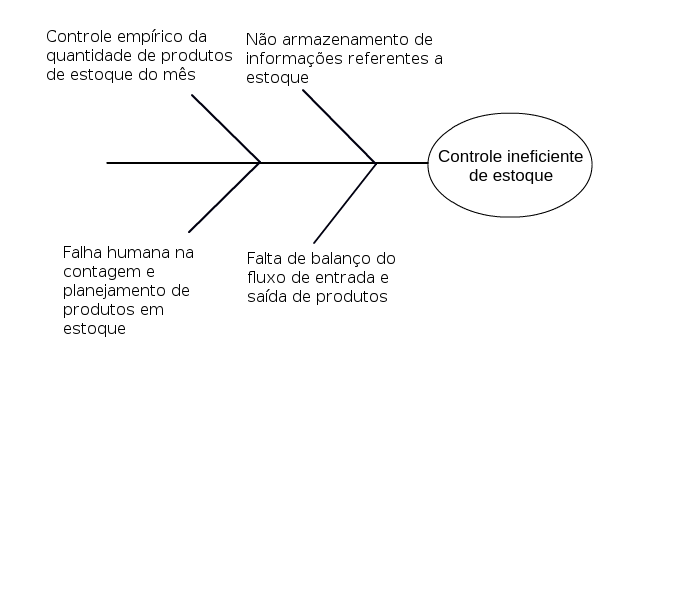
\includegraphics[scale=0.45]{figuras/analise_do_problema/fishbone_problema1}
		\caption{Diagrama espinha de peixe - Controle de estoque ineficiente}
\end{figure}

\subsection{Falta de controle de desperdício na produção}

\begin{figure}[!htpb]
		\centering
		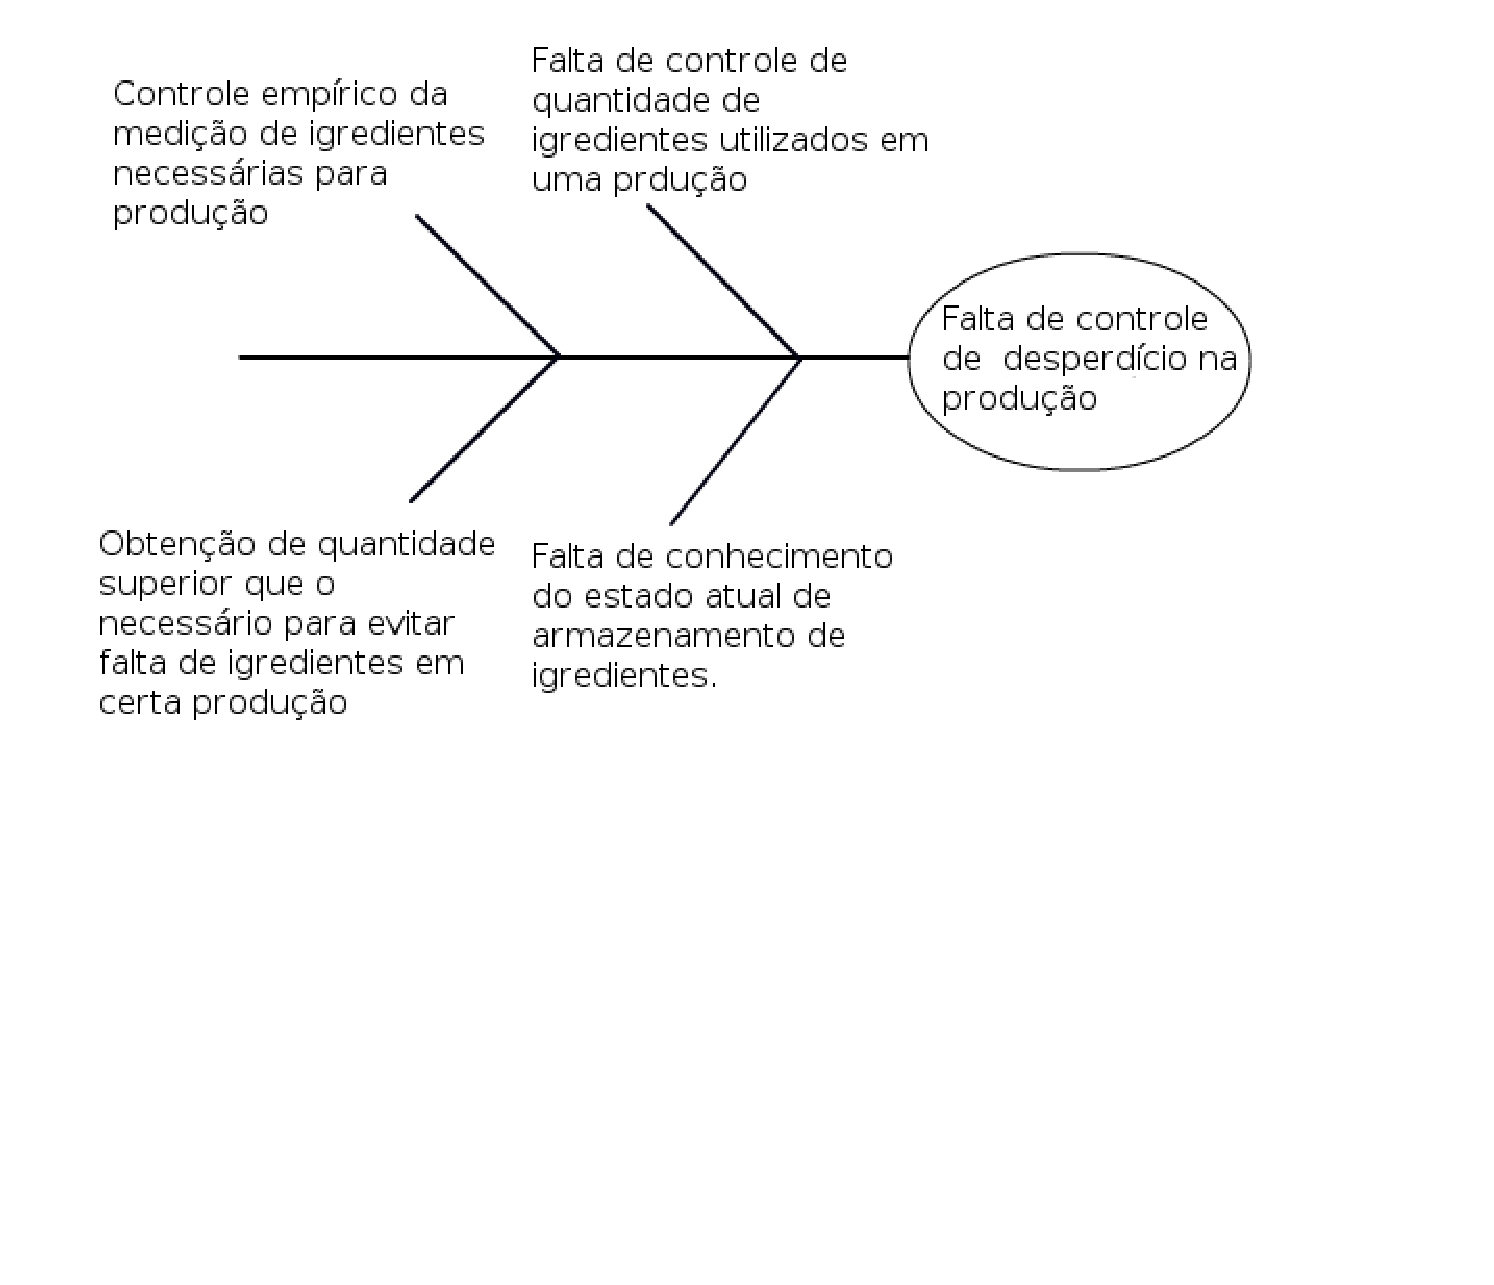
\includegraphics[scale=0.45]{figuras/analise_do_problema/fishbone_problema2}
		\caption{Diagrama espinha de peixe - Falta de controle de desperdício na produção}
\end{figure}
